
\frame{
  \frametitle{Analyse}
  Cibles visées
    \begin{itemize}
      \item Réseau interne.
      \item Navigateurs web:
        \begin{itemize}
          \item Chrome 44\%
          \item Firefox 19\%
        \end{itemize}
    \end{itemize}
   Protocole SSL/TLS
     \begin{itemize}
       \item Protocole de sécurisation des échanges
       \item Mode client/serveur
       \item Authentification, confidentialité, intégrité
       \item Fragmentation des données
       \item HMAC pour l'intégrité
     \end{itemize}
}

\frame{
  \frametitle{Analyse}
     Record TLS
       \begin{itemize}
         \item Envoi: message-fragmentation-compression-HMAC-chiffrement
         \item Réception: déchiffrement-décompression-rassemblement
       \end{itemize}
     Handshake
       \begin{itemize}
         \item Négocier une session TLS
         \item Eléments d'une session
           \begin{itemize}
             \item session identifier
             \item peer certificate
             \item compression method
             \item cipher spec
             \item master secret
             \item Is resumable
           \end{itemize}
       \end{itemize}
}

\frame{
  \frametitle{Analyse}
  Etapes du Handshake
  \begin{enumerate}
    \item Client Hello
    \item Server Hello
    \item Server Certificate
    \item Client Key Exchange
    \item Change Cipher Spec
  \end{enumerate}
  
}

\frame{
  \frametitle{Conception}
  UML des classes Java
  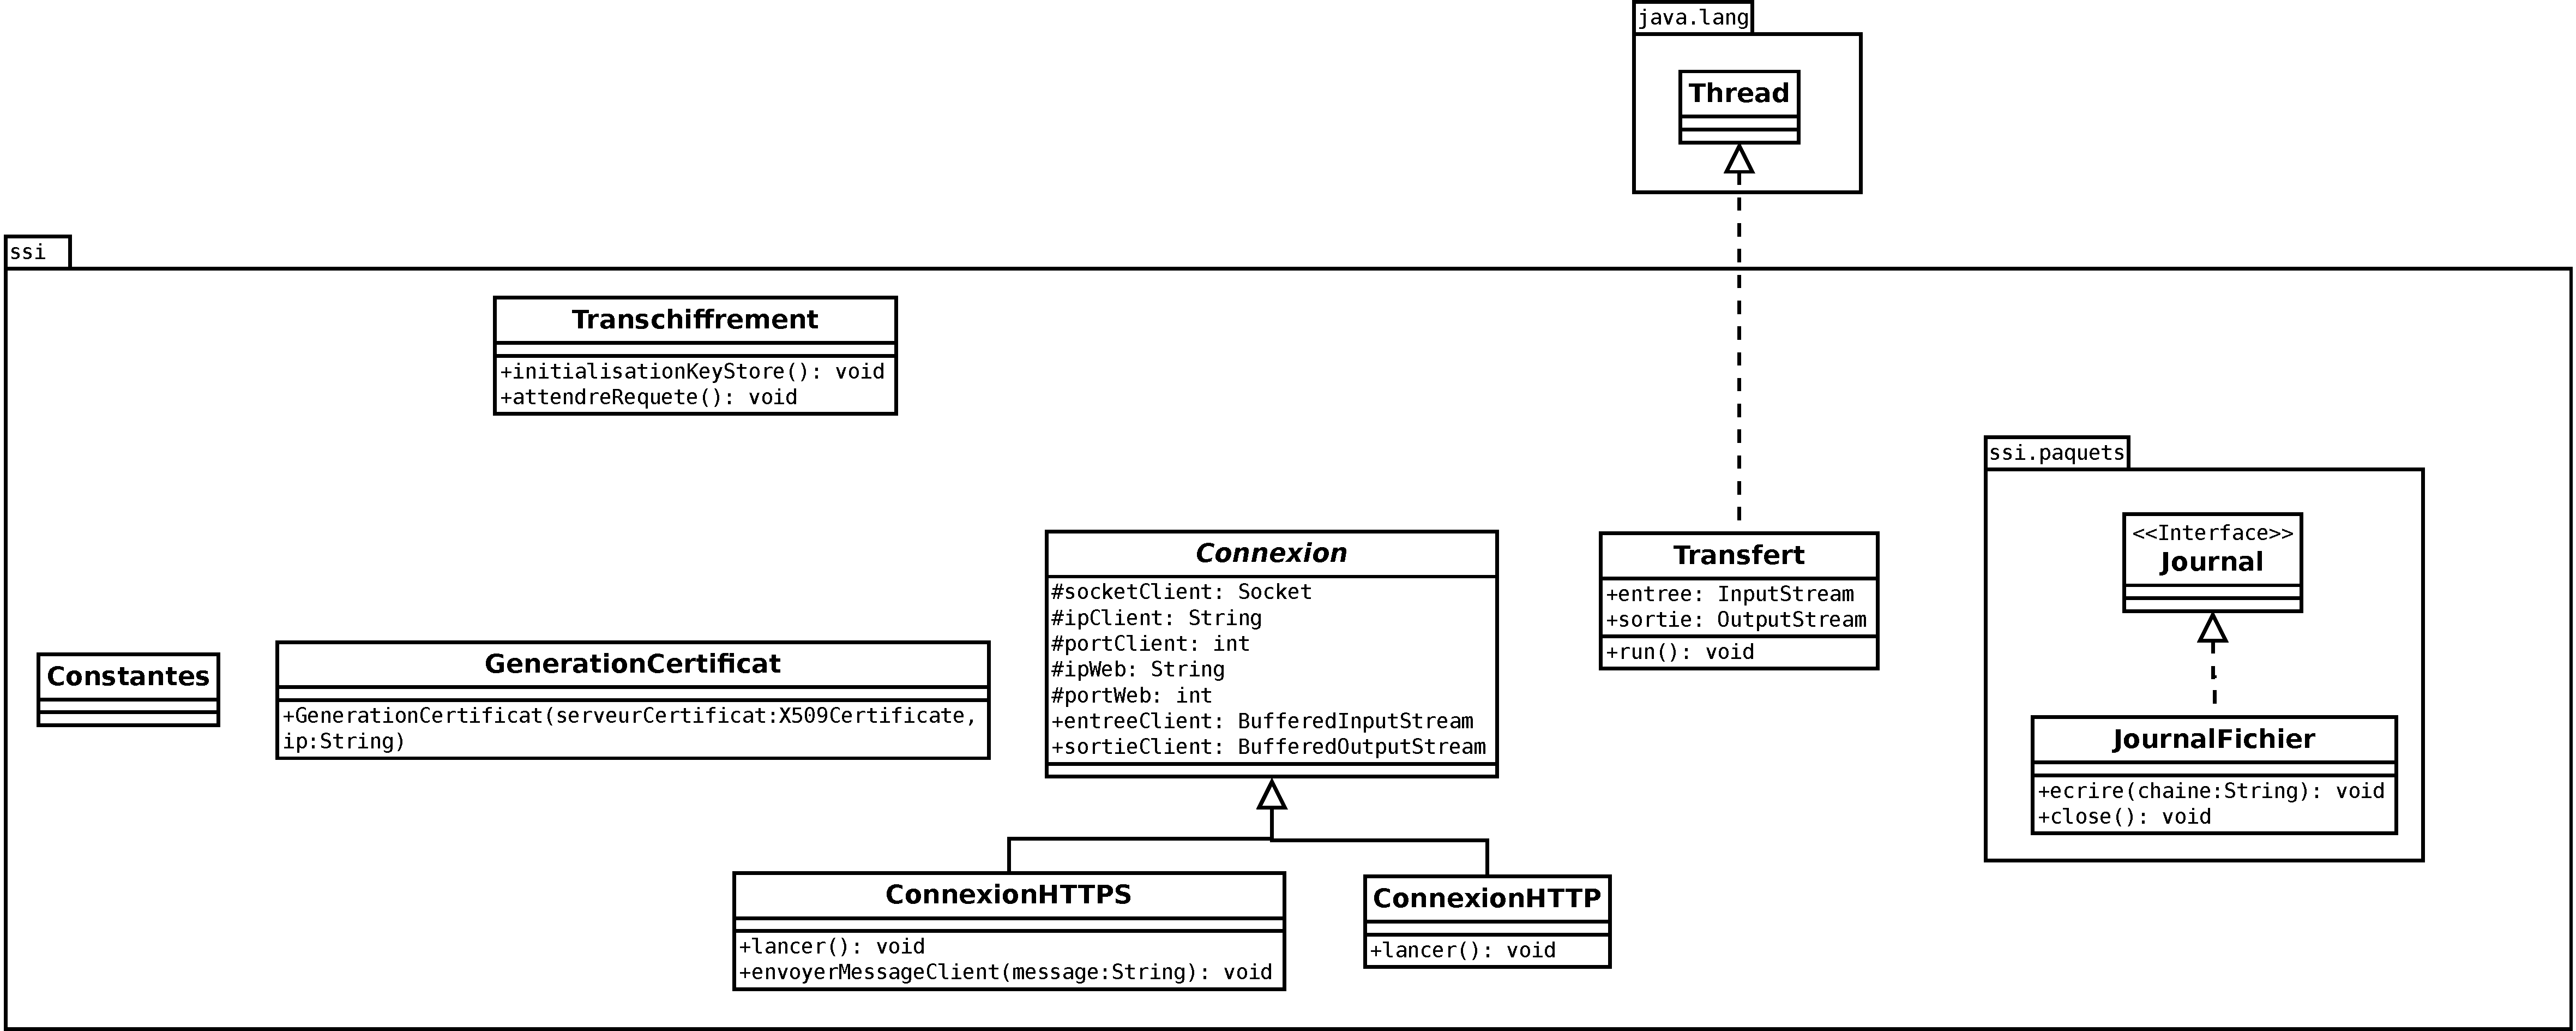
\includegraphics[width=\textwidth]{text/uml.pdf}
}

\frame{
  \frametitle{Accepter une autorité}
  Installer une autorité
  \begin{itemize}
    \item Utilisation d'un script
    \item Directement sur la machine utilisateur
    \item Dans le navigateur web du client
    \item Collision MD5
  \end{itemize}
  
  Collision MD5, vue d'ensemble
  \begin{itemize}
    \item Forge d'un faux certificat
    \item Signature identique
    \item Eviter l'installation d'une autorité
    \item Transparence maximale
  \end{itemize}
  
}
